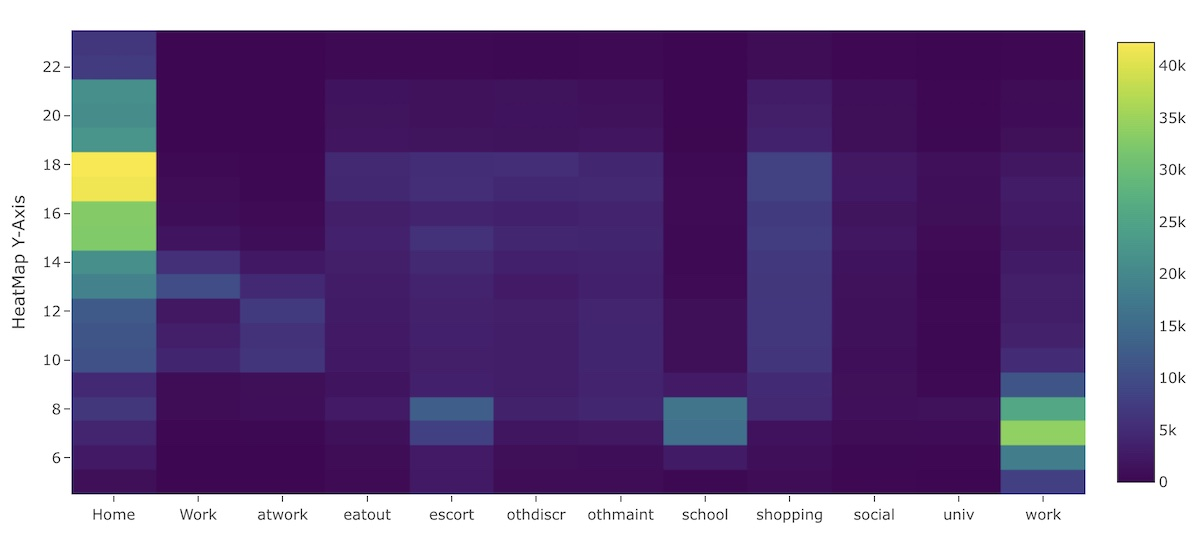
\includegraphics{assets/heatmap-chart.jpg} \emph{Heatmap depicting Time
of day vs.~activity purpose}

A heatmap chart depicts aggregate data in two dimensions on one chart.

\hypertarget{usage}{%
\subsection{Usage}\label{usage}}

Heatmap charts can only be included as panels in \textbf{Dashboards}.
See Dashboard documentation for general tips on creating dashboard
configurations.

\begin{itemize}
\tightlist
\item
  Use panel \texttt{type:\ heatmap} in the dashboard configuration.
\item
  Each heatmap panel is defined inside a \textbf{row} in a
  \texttt{dashboard-*.yaml} file.
\item
  Standard title, description, and width fields define the frame.
\end{itemize}

\begin{center}\rule{0.5\linewidth}{0.5pt}\end{center}

\hypertarget{sample-dashboard.yaml-config-snippet-with-a-heatmap}{%
\subsubsection{Sample dashboard.yaml config snippet with a
heatmap}\label{sample-dashboard.yaml-config-snippet-with-a-heatmap}}

\begin{Shaded}
\begin{Highlighting}[]
\FunctionTok{layout}\KeywordTok{:}
\AttributeTok{  }\FunctionTok{row1}\KeywordTok{:}
\AttributeTok{    }\KeywordTok{{-}}\AttributeTok{ }\FunctionTok{title}\KeywordTok{:}\AttributeTok{ }\StringTok{"My Heatmap"}
\AttributeTok{      }\FunctionTok{type}\KeywordTok{:}\AttributeTok{ heatmap}
\AttributeTok{      }\FunctionTok{dataset}\KeywordTok{:}\AttributeTok{ }\StringTok{"trips{-}tod{-}wide.csv"}
\AttributeTok{      }\FunctionTok{y}\KeywordTok{:}\AttributeTok{ depart}
\AttributeTok{      }\FunctionTok{columns}\KeywordTok{:}\AttributeTok{ }\KeywordTok{[}\StringTok{\textquotesingle{}Home\textquotesingle{}}\KeywordTok{,}\StringTok{\textquotesingle{}Work\textquotesingle{}}\KeywordTok{,}\StringTok{\textquotesingle{}atwork\textquotesingle{}}\KeywordTok{,}\StringTok{\textquotesingle{}eatout\textquotesingle{}}\KeywordTok{,}\StringTok{\textquotesingle{}escort\textquotesingle{}}\KeywordTok{,}\StringTok{\textquotesingle{}othdiscr\textquotesingle{}}\KeywordTok{,}\StringTok{\textquotesingle{}othmaint\textquotesingle{}}\KeywordTok{,}
\AttributeTok{                }\StringTok{\textquotesingle{}school\textquotesingle{}}\KeywordTok{,}\StringTok{\textquotesingle{}shopping\textquotesingle{}}\KeywordTok{,}\StringTok{\textquotesingle{}social\textquotesingle{}}\KeywordTok{]}
\AttributeTok{      }\FunctionTok{xAxisTitle}\KeywordTok{:}\AttributeTok{ }\StringTok{"Activity Purpose"}
\AttributeTok{      }\FunctionTok{yAxisTitle}\KeywordTok{:}\AttributeTok{ }\StringTok{"Time of Day (Hour)"}
\AttributeTok{      }\FunctionTok{flipAxes}\KeywordTok{:}\AttributeTok{ }\CharTok{true}
\end{Highlighting}
\end{Shaded}

\begin{center}\rule{0.5\linewidth}{0.5pt}\end{center}

\hypertarget{heatmap-chart-properties}{%
\subsubsection{Heatmap chart
properties}\label{heatmap-chart-properties}}

Heatmap chart properties:

\textbf{dataset:} String. The filepath containing the data. May include
wildcards * and ?.

\textbf{y:} column containing y-value data.

\textbf{columns:}: Array{[}{]} containing names of columns with data to
be categorized on the x-axis. See example above.

\textbf{xAxisTitle} and \textbf{yAxisTitle}: Descriptive titles for the
x-axis and y-axis (optional).

\textbf{flipAxes:} True/false. Transpose the heatmap matrix, thus
flipping the x and y axes. Can be useful if your data is stored one way
but you want it displayed the other.
